\section{Resultados}

\subsection{Resultados de investigación}

En esta sección se exponen los conceptos, lecciones y conclusiones más relevantes del proceso de investigación seguido como base para la posterior experimentación.

A diferencia del capítulo anterior donde razonábamos el Estado del Arte desde la perspectiva de lo interesante para las preguntas de investigación, aquí se exponen otros elementos que se han considerado necesarios comprender.

\subsubsection{Conceptos generales}

\paragraph{Atención} ~\\

Una de las primeras cosas que llamaron nuestra atención en la medida que se profundizaba en aspectos más técnicos de algunos de los modelos generadores de voz fue el concepto de atención. En términos generales entendemos atender como el acto de tomar en consideración a alguien o a algo particular respecto al resto al resto del entorno. 

Este concepto se aplica también al ámbito del Aprendizaje Computacional. En primer lugar es necesario aclarar que en general el entrenamiento de un modelo a partir de un conjunto de datos ya supone en cierto grado diferenciar la información relevante de aquella que no es significativa. Cuando hablamos de forma explícita de paradigmas o mecanismos de atención en un modelo determinado hablamos de forzar por diseño el peso de cierta parte de la información frente a otra.

Algunos modelos implementan mecanismos de atención especialmente relevantes, como los Transformer que se han hecho especialmente populares en años recientes en muchos problemas del procesamiento natural del lenguaje\footnote{Aunque no parece ser el caso en la síntesis de voz, pues la propuesta de Transformer TTS no obtuvo muy buenos resultados comparado con otras propuestas}.

Dependiendo de la forma de actuar de los diferentes mecanismos de atención podemos distinguir entre atención y auto-atención, siendo esta última bastante relevante en el modelo que hemos comentado:

\begin{displayquote}
«Self-attention, sometimes called intra-attention is an attention mechanism relating different positions of a single sequence in order to compute a representation of the sequence. Self-attention has been used successfully in a variety of tasks including reading comprehension, abstractive summarization, textual entailment and learning task-independent sentence representations»\hyperref[RES_1]{[14]}
\end{displayquote}

Debemos comprender que en los modelos tratados tenemos una entrada de datos como secuencia de longitud variable y una salida igualmente de longitud variable, esto se aborda con una arquitectura codificador-decodificador donde un mecanismo de atención es esencial.

Tacotron 2 emplea un mecanismo de atención especial basado en localización en la secuencia y en información temporal de pasos previos:

\begin{displayquote}
«We use the location-sensitive attention [...] which extends the additive attention mechanism to use cumulative attention weights from previous decoder time steps as an additional feature.»
\end{displayquote} \hyperref[EA_6]{[8]}

Por su parte VITS emplea el mismo mecanismo de atención de otro modelo anterior publicado por el mismo grupo de investigadores, llamado Glow-TTS \hyperref[RES_1]{[15]}:

\begin{displayquote}
«We follow the encoder structure of Transformer TTS with two slight modifications. We remove the positional encoding and add relative position representations into the self-attention modules instead»
\end{displayquote}

\paragraph{Alineamiento} ~\\

En los modelos basados en la arquitectura codificador-decodificador se precisa transformar una entrada de datos de longitud variable en una representación intermedia de tamaño fijo (codificar) para posteriormente transformar esta representación en una salida de tamaño variable (decodificar).

Durante el entrenamiento del modelo uno de los principales objetivos es encontrar la adecuada representación intermedia de los datos, encontrando en esa representación la relación entre la entrada y salida de datos. Este proceso es el que denominamos alineamiento en el modelo.

La evaluación de este alineamiento es una de las cosas que se ha tenido que prestar atención en el entrenamiento de los modelos, especialmente en el caso de Tacotron 2 que es menos robusto en ese sentido.

\begin{figure}[H]
\centering
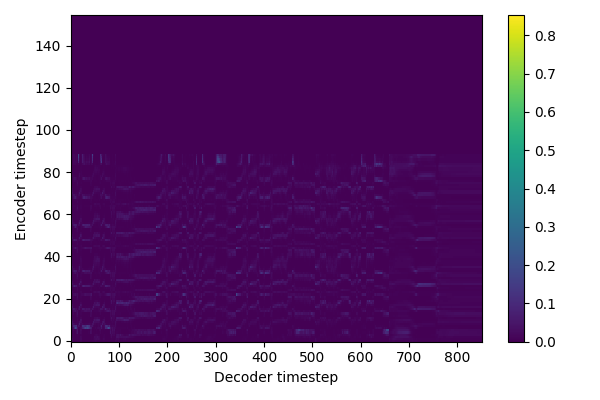
\includegraphics[width=10cm]{5_resultados_img/align-taco1.png}
\caption{Falta de alineamiento en un entrenamiento de Tacotron 2}
\label{fig:figure1}
\end{figure}

En esta figura podemos ver una fase muy temprana de entrenamiento de Tacotron 2 donde la representación intermedia de los datos es difusa.

\begin{figure}[H]
\centering
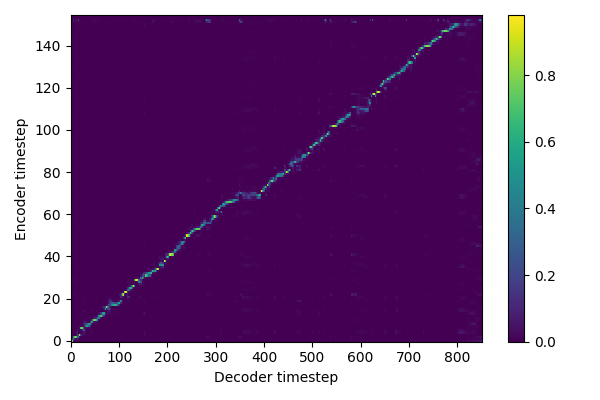
\includegraphics[width=10cm]{5_resultados_img/align-taco2.png}
\caption{Alineamiento definido en un entrenamiento de Tacotron 2}
\label{fig:figure1}
\end{figure}

El entrenamiento posteriormente progresó a un alineamiento notable, este es el resultado esperable pare el modelo Tacotron 2 con su arquitectura encoder-decoder particular.

\begin{figure}[H]
\centering
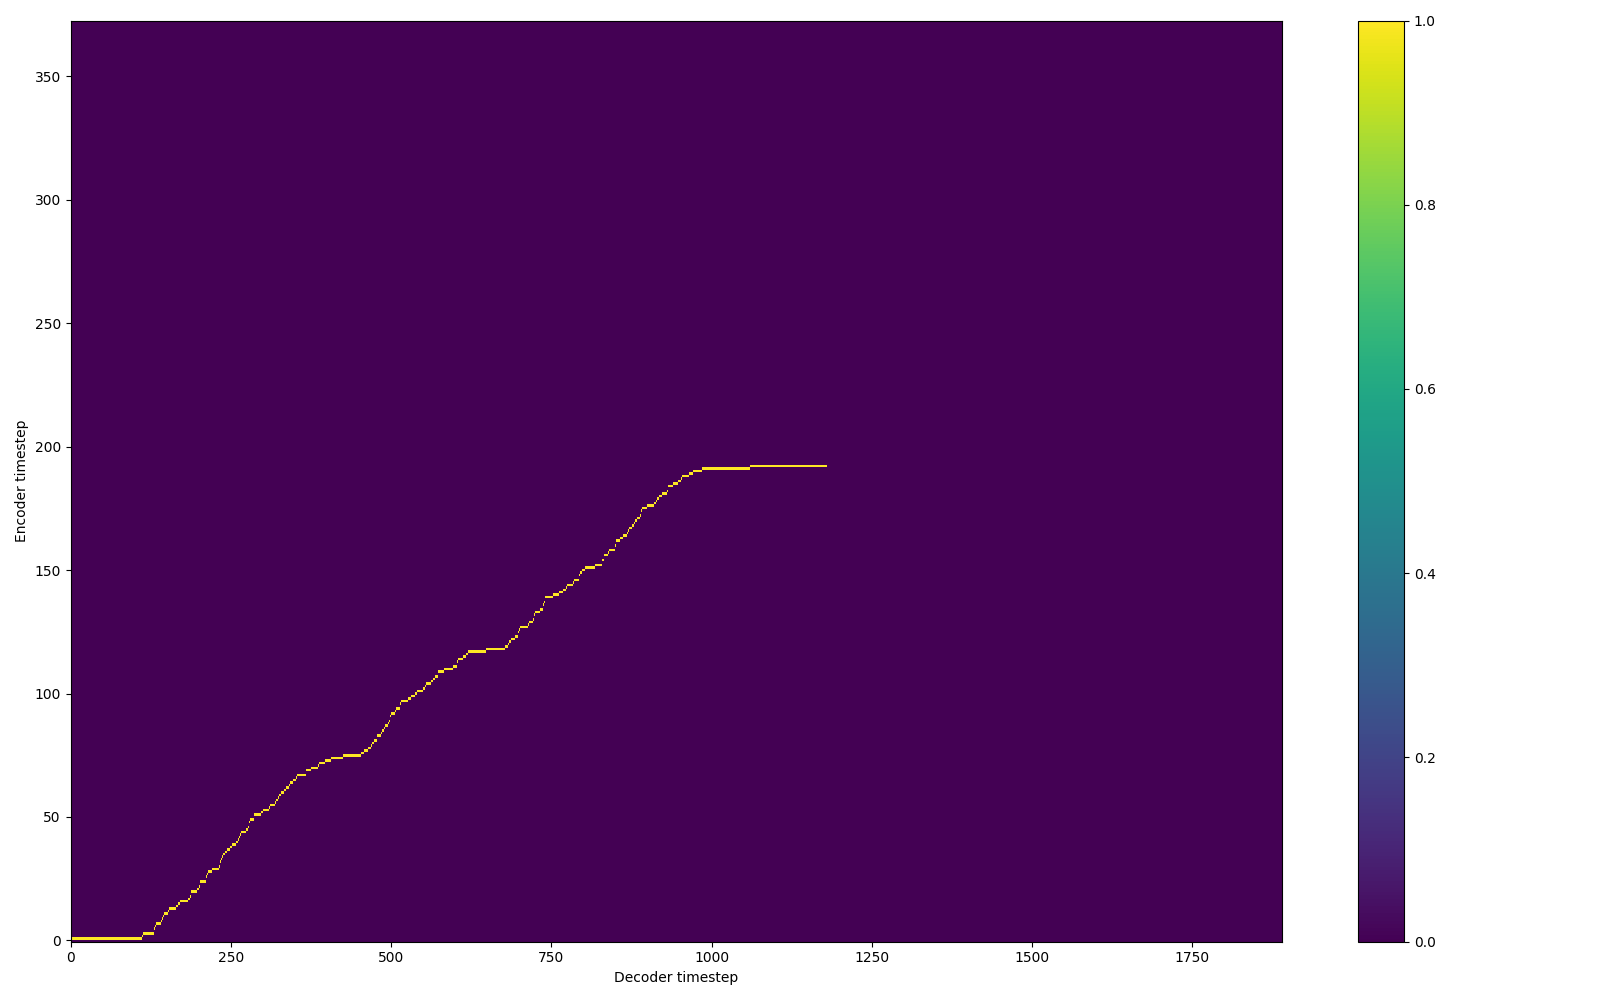
\includegraphics[width=10cm]{5_resultados_img/align-vits.png}
\caption{Alineamiento muy definido en el modelo VITS}
\label{fig:figure1}
\end{figure}

En este caso podemos ver como VITS es mucho más robusto en este aspecto, teniendo un alineamiento claramente definido.

\paragraph{Escala MOS} ~\\

Para todo problema que se aborda existe la necesidad de definir una escala que permita evaluar el grado de cumplimiento. En la mayoría de modelos estudiados esta métrica es la escala MOS (Mean Opinion Score), una métrica heredada de los sistemas de telefonía.

La escala MOS intenta medir la calidad de una comunicación de voz mediante la opinion media de los usuarios, su origen está en una recomendación de la International Telecomunication Union (ITU) publicada como P.800.1 \hyperref[RES_3]{[17]}.

En ella se define la escala como: 

\begin{displayquote}
«The value on a predefined scale that a subject assigns to his opinion of the performance of the telephone transmission system used either for conversation or for listening to spoken material»
\end{displayquote}

En la publicación también se comenta la posibilidad de definir la escala de forma objetiva, pero en los modelos revisados o no se dan más detalles del uso de esta escala o se comenta que se ha realizado una encuesta con muestras generadas.

Aunque esta escala nos ayuda a comprender las posibilidades de un modelo para generar voz de calidad no nos permite medir la calidad con la que el modelo imita la voz original del hablante y en qué grado permitiría generar una falsificación.

\subsubsection{Componentes y arquitecturas}

\paragraph{Modelos basados en RNN}

En el campo del Aprendizaje Computacional existen cada día más modelos y componentes de modelos distintos. El campo avanza a pasos agigantados cubriendo cada vez más categorías de problemas y encontrando mejores soluciones a problemas ya cubiertos con anterioridad.

En muchos problemas abordados el tamaño de la entrada de datos es fija o cuanto menos es fácilmente transformable a una entrada da datos normalizada sin perder información. Por ejemplo, en muchos problemas de Visión por Computador se traducen las imágenes a unas dimensiones determinadas en las cuales ha sido entrenado el modelo. 

En el caso de problemas de procesamiento natural del lenguaje, la entrada de datos es siempre de longitud variable y no existe una forma sencilla de preprocesar los datos para dimensionarlos a un tamaño fijo.


\begin{figure}[H]
\centering
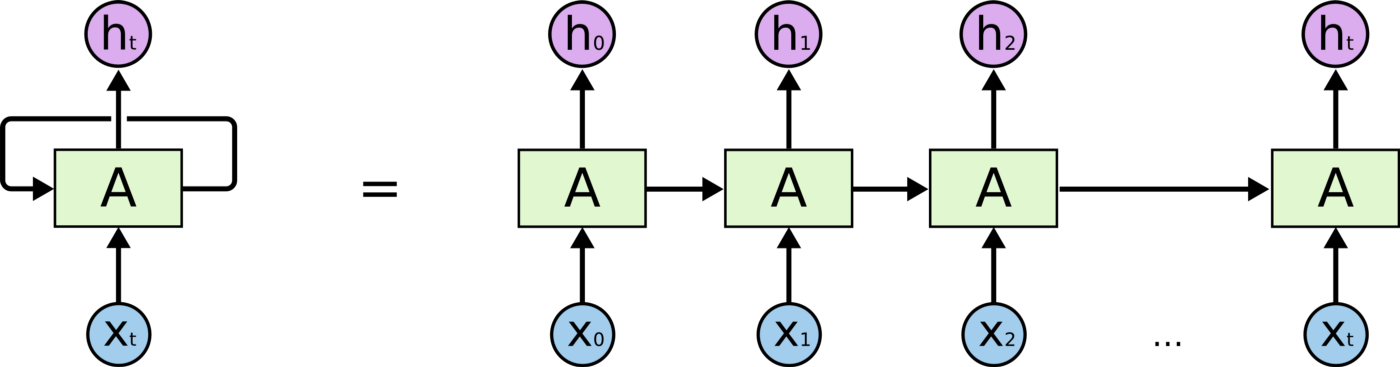
\includegraphics[width=10cm]{5_resultados_img/rnn-1.png}
\caption{Modelo RNN y su despliegue en un modelo secuencia.}
\label{fig:figure1}
\end{figure}

El uso modelos basados en redes neuronales recurrentes se vuelve entonces poco práctico \hyperref[RES_2]{[16]}, pues la complejidad de la red crece con el tamaño de la entrada de datos. Se hace necesario encontrar otras arquitecturas que puedan manejar la arbitrariedad del tamaño de los datos.

\paragraph{Modelos Codificador-Decodificador}

Se han mencionado ya varias veces con anterioridad para comentar características particulares o valoraciones del entrenamiento de algunos modelos, pero no hemos comentado en detalle lo que suponen los modelos codificador-decodificador (en inglés encoder-decoder o E/D). 

Partimos de una entrada de datos de longitud arbitraria, habitualmente una oración completa que traducir, analizar sentimientos, sintetizar voz o cualquier otra tarea similar. Si empleamos alguna arquitectura sencilla con perceptones y redes conectadas de forma simple, tendríamos que redimensionar la entrada de datos a un tamaño fijo con el cual el modelo ha sido entrenado. En otros modelos entenderíamos ese paso como una fase de normalización de los datos.

Pero no existe ninguna forma sencilla de normalizar información en formato textual a una dimensionalidad determinada y una expresión única. Tenemos además el problema añadido de que el lenguaje natural tiene múltiples formas de expresar información equivalente. Es cierto que existen formas matemáticas\footnote{Habitualmente en modelos que tienen vectores de N dimensiones donde cada palabra tiene un valor para cada dimensión del vector. Por ejemplo GloVe o word2vec son modelos así.} de representar palabras, por ejemplo haciendo uso de word embeddings, pero si combinamos los valores en un vector final la información se va diluyendo.

\begin{figure}[H]
\centering
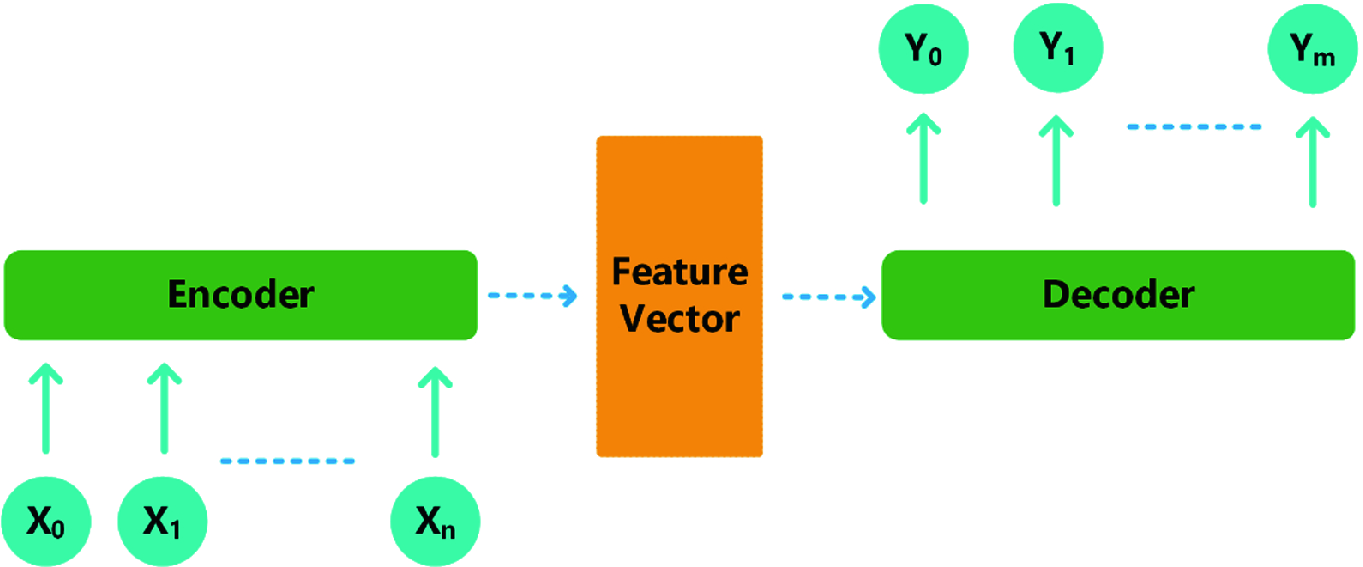
\includegraphics[width=14cm]{5_resultados_img/e-d.png}
\caption{Representación abtracta de un modelo codificador-decodificador.}
\label{fig:figure1}
\end{figure}

Necesitamos alguna forma de identificar la información más relevante en una oración determinada y al mismo tiempo mapear esa información a un estado oculto intermedio en el modelo. Ese es el paradigma de estos modelos codificador-decodificador, pero la forma en la cual se mapea esa información en un estado intermedio es un nuevo problema que puede tener muchas soluciones.

Dentro de las soluciones a este problema precisamente aparecen los dos conceptos que hemos definido anteriormente: atención y alineamiento. Un mecanismo de atención lo que nos permite es representar la información relevante en una entrada de forma y longitud variable. Para ello podemos confiar en las relaciones entre las diferentes palabras (auto-atención) o en otras cuestiones de localización o temporalidad de la entrada de la secuencia de datos (atención).

Muchos de los cambios y avances de los modelos revisados parten de revisar y abordar este problema desde una perspectiva distinta o con ajustes añadidos. 

Como habíamos comentado más arriba, durante el proceso de entrenamiento de estos modelos, una de las métricas que debemos observar para evaluar el avance del entrenamiento es el alineamiento. Esto implica que efectivamente conseguimos representar la información de entrada fielmente en el estado intermedio y que el decodificador consigue reconstruir a partir de esta representación la salida esperada del modelo.

\subsubsection{Datasets}

Para realizar el entrenamiento de los modelos contemplados es necesario conseguir datos del perfil de voz de la persona en un formato particular. Ninguno de los modelos abordados contempla el uso de conjuntos de datos de más de un hablante, por lo que nos ceñiremos a los datasets de una sola persona.

Los datos en este dataset deben presentarse como una serie de parejas de sonido y su transcripción textual en el idioma que se aborde. El formato particular para realizar el emparejamiento varía, aunque es habitual que se presente como un conjunto de clips de sonido y un fichero de datos CSV o TSV que los empareja con su transcipción.

Las características de estos datasets pueden determinar en gran medida el éxito del entrenamiento del modelo. El proyecto Mozilla TTS \hyperref[RES_4]{[18]} lista los siguientes puntos de atención para obtener un dataset de buena calidad:

\begin{itemize}
    \item Variedad en longitud de los fragmentos de audio: se sugiere una distribución gaussiana de la longitud de los clips.
    \item Ausencia de errores de transcripción: coincidencia entre los fonemas vocalizados y su representación textual en esa lengua.
    \item Grabaciones de calidad sin ruido: claridad, falta de distorsión, sonidos de fondo o ruido base.
    \item Tono y velocidad homogéneos entre clips: pronunciación neutra y constante en todos los fragmentos.
    \item Adecuada cobertura de fonemas: deben incluirse muestras que cubran todos los fonemas posibles del idioma.
    \item Naturalidad: pausas y entonación adecuada.
\end{itemize}

Algunas de estas características se han tenido especialmente en cuenta, otras de las recomendaciones son demasiado subjetivas para poder cuantificarse y especialmente para cuantificarse entre diferentes idiomas.

Se han generado algunas métricas concretas de varios datasets que se encuentran en el anexo \hyperref[Análisis de datasets]{Análisis de datasets}.

\subsubsection{Herramientas comerciales}

Algunas herramientas comerciales que hacen uso de algunas características de estos modelos han ido apareciendo con el tiempo, pero no suelen cumplir la función de síntesis de voz entrenable que realmente cuadra con los objetivos del proyecto.

De las diversas herramientas y webs probadas, prácticamente ninguna realmente ofrece algo adaptable, únicamente Resemble.ai ofrece algo similar. Esta web promete un modelo de voz luego de haber grabado 50 fragmentos de audios mediante su interfaz. El problema es que únicamente acepta inglés como idioma en su versión gratuita.

Otra web que ofrece algunas características prometedoras es fakeyou.com, quizá lo más cercano a lo que hemos investigado y experimentado, pero no se ha llegado a profundizar en el uso de esta web ya que se encontraron problemas con ella durante las pruebas de uso. 

Esta web sí que positivamente lista en la descripción de su misión y funcionamiento alguno de los modelos que hemos estudiado, como Tacotron 2.

\subsection{Resultados de experimentación}

En este apartado entramos a detallar los resultados de los diferentes experimentos realizados, tanto en lo positivo como en los errores, fallos y limitaciones encontrados en el proceso.

\subsubsection{Datasets}

Aunque existen ya datasets de voz en castellano con los que algunos de los modelos vistos se han podido entrenar, para conseguir el objetivo de entrenar un modelo con la voz propia se ha decidido generar un dataset propio.

Se ha intentado mantener cierta homogeneidad en el tiempo de los fragmentos, pues el tamaño de los mismos condiciona las necesidades de memoria en el entrenamiento de los modelos y unos tiempos cercanos aseguran que el entrenamiento podrá aprovechar al máximo los recursos de hardware sin eventualmente encontrar errores por falta de memoria.

Algunos detalles más técnicos sobre la grabación de audio se puede localizar en el \hyperref[Grabación de datasets]{Anexo 11.1}. El resultado final en forma de dataset se encuentra documentado en la sección \hyperref[Entregables]{8. Entregables}.

\paragraph{Primera iteración} ~\\

En una primera iteración de la generación de este dataset y posteriormente su uso como datos de entrenamiento se identificaron varios problemas. El más importante de ellos fue la ausencia de ciertos fonemas en el conjunto de entrenamiento. 

No se usó ningún criterio particular para la selección de los fragmentos de texto a grabar y como era esperable en cierto grado se reprodujo la tabla de frecuencias de los fonemas del castellano. El problema de esto es que ciertos sonidos le costarían mucho al modelo aprenderlos o no los aprendería en absoluto.

Adicionalmente en esta primera prueba apenas se grabaron 30 minutos de audio en 130 fragmentos, lo que hacía que la muestra de fonemas fuese aún más pobre en algunos casos.

\paragraph{Segunda iteración} ~\\

En esta segunda iteración se emplearon técnicas similares a las anteriormente mencionadas pero se tuvo especial atención al ruido ambiental. Se hizo manifiesto que este ruido se trasladaba a los resultados del modelo y en algunos casos se amplificaba haciéndose mucho más notable. 

Además de buscar un entorno menos ruidoso se incorporaron mecanismos de redacción de ruido adicionales con lo que la calidad mejoró.

Se grabaron un total de 500 frases y se amplió la longitud máxima de las mismas a 50 palabras (anteriormente se había fijado en 24) esperando así mejorar la inferencia de textos más largos.

Adicionalmente se optó por mantener las grabaciones de sonido con la calidad original de muestreo de 48kHz en lugar de 22kHz que es la habitual en estos datasets destinados al entrenamiento de modelos de síntesis de voz.

\subsubsection{Modelos}

En la revisión del estado del arte se identificaron muchos modelos distintos susceptibles de ser probados y entrenados con el dataset de voz propio que se estaba generando, pero el entrenamiento de modelos resulta costoso en tiempo y recursos.

En general el tiempo de entrenamiento de cada modelo ha variado entre 3 días y una semana en local y siempre más de una semana en Google Colab. Sobre las dificultades para entrenar modelos en Google Colab y las posibles soluciones se ha redactado un \hyperref[Entrenamiento en Google Colab]{anexo específico}.

Esto ha supuesto la obligación de elegir un solo modelo en el que centrar el grueso del tiempo y recursos disponibles para este trabajo. El modelo finalmente elegido fue VITS por posicionarse como el que mejores resultados ofrece con los datos actuales y que al mismo tiempo tenga una implementación abierta.

Antes de que se tomase esta decisión se comenzaron a hacer pruebas de entrenamiento con Tacotron 2 poco satisfactorias, aunque también se considera relevante documentarlo.

\paragraph{Tacotron 2} ~\\

En una etapa temprana de desarrollo del proyecto se comenzó a revisar el código del modelo Tacotron 2 en la implementación que NVIDIA había hecho pública \hyperref[RES_5]{[19]}. Se encontraron bastantes problemas por incompatibilidades de software.

Todo el código que se ha trabajado en este trabajo se ha realizado en Python y empleando algunas librerías para Aprendizaje Computacional como son TensorFlow o (Py)Torch. Para que el software de un modelo funcione adecuadamente tiene que existir compatibilidad entre estos elementos:

\begin{enumerate}
    \item Intérprete de Python
    \item Implementación del modelo en código
    \item Librerías que use la implementación
    \item Lenguaje/arquitectura de aceleración
    \item Drivers de la GPU
    \item GPU
\end{enumerate}

En proyectos cuyo código se encuentra adecuadamente mantenido no suele haber problemas, pero este proyecto había publicado su implementación hace unos 4 años y no se ha mantenido demasiado actualizado el código en línea con las dependencias que tenía.

Particularmente encontramos que la versión de Torch que se instala por defecto al instalar los requisitos del repositorio no es compatible con la GPU del sistema. Fue necesario instalar una versión especial que sí implementa compatibilidad con las últimas tarjetas gráficas de NVIDIA. Más detalles sobre esto se encuentran en el anexo \hyperref[Entorno de entrenamiento]{Entorno de entrenamiento}.

Una vez subsanados los problemas más técnicos se inició un entrenamiento con el dataset LJSpeech, que progresivamente devolvió resultados aceptables de síntesis de voz


\paragraph{VITS} ~\\

En términos de experimentación gran parte del esfuerzo se volcó en este modelo, habiéndose realizado con él numerosos experimentos. En un primer momento se hizo revisión de la base de código originalmente publicada \hyperref[RES_6]{[20]} por los autores del modelo, pero finalmente se trabajó con la implementación del toolkit Coqui-AI.

Una de la primeras cosas que nos dimos cuenta trabajando con este modelo fue la robustez con la que se progresaba hacia un alineamiento muy definido, algo que había sido relativamente problemático con Tacotron 2 como se había comentado más arriba cuando hablábamos de este concepto.

\begin{figure}[H]
\centering
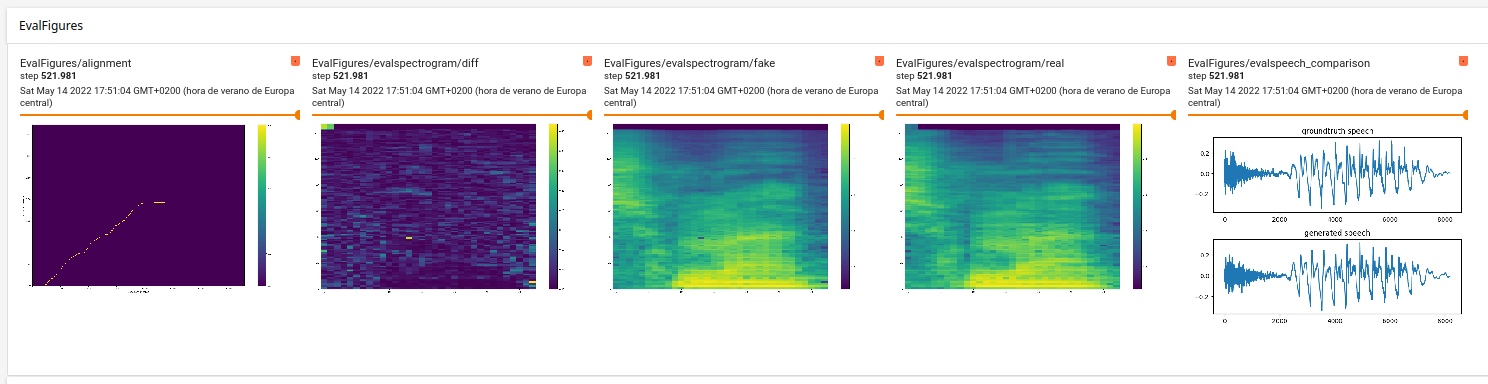
\includegraphics[width=14cm]{5_resultados_img/vits-2.png}
\caption{Alineamiento junto a otras métricas en TensorBoard.}
\label{fig:figure1}
\end{figure}

Durante los entrenamientos el seguimiento del progreso se ha realizado empleando una herramienta llamada TensorBoard, que permite visualizar la progresión de algunos estados internos del modelo, métricas y muestras de generación. Los registros de estos entrenamientos se presentan también como entregables.

Una vez que pudimos reproducir los resultados de entrenamiento en inglés comenzamos a hacer los ajustes necesarios en el modelo para poder trabajar con castellano. Entre los cambios se incluyen:

\begin{itemize}
    \item Ampliar la lista de caracteres reconocidos por el modelo
    \item Ajustar la lista de fonemas posibles
    \item Ajustar el reemplazo de ciertos caracteres especiales por su nombre
\end{itemize}

Parte de este trabajo se puede encontrar en un \href{https://github.com/daniel-dona/coqui-ai-TTS}{fork} específico del repositorio de Coqui-AI.

Con ello se pudo realizar un primer entrenamiento cuando el dataset aún contenía poco más de 100 registros grabados. En este punto existían aún bastantes errores de síntesis en ciertas palabras, aunque en cambio otras se sintetizaban sin problema. En este punto empezamos a sospechar la posibilidad de que se estuviesen generando fonemas en las inferencias que no estaban en el dataset\footnote{Algunos elementos más sobre esto se encuentran en el anexo sobre Análisis de Datasets}.

Una vez se generó el dataset más amplio de 500 registros se consiguieron resultados bastante mejores, sin apenas errores de pronunciación en las inferencias generadas. A partir de ese momento se comenzó a valorar el realizar ajustes de hiperparámetros del modelo en la búsqueda de obtener aún mejores resultados.

Se valoraron los siguientes parámetros:

\begin{itemize}
    \item Tamaño de lote y tasa de aprendizaje
    \item Canales MEL y frecuencia de muestreo
    \item Fonetizador
\end{itemize}

El primer parámetro fue de ajuste obligado pues la GPU empleada en la mayoría de entrenamientos (local) solo disponía de 12GB de memoria y no toda disponible. El tamaño de lote es un valor que ajusta cuántas muestras del dataset se cargan y procesan de forma simultánea.

Un problema encontrado al realizar este ajuste es que el tamaño ocupado en memoria no es siempre el mismo, al variar la longitud de los registros de audio, por lo que debemos establecer valores prudentes. A la par que reducimos el tamaño de lote debemos ajustar de forma acorde la tasa de aprendizaje, pues estamos modificando los pasos de entrenamiento del modelo.

También hay que tener en cuenta que este modelo ajusta dinámicamente la tasa de aprendizaje según progresa el entrenamiento, nosotros solo establecemos un valor inicial. En general este valor no es crítico, un valor muy alto puede hacer que el modelo apenas progrese y un valor muy bajo puede hacer que el entrenamiento caiga en un mínimo local del que no pueda salir, pero existe un rango de valores que posiblemente funcionen y permitan un buen entrenamiento.

El siguiente parámetro define una representación interna del modelo, posterior al decodificador, que emplea espectrogramas MEL como forma de representación del sonido generado. Esta es la representación que consumirá el vocoder (sea externo o integrado en el modelo) y a partir de donde se generará la forma de onda final.

Un espectrograma MEL se caracteriza por emplear diferentes filtros por bandas de frecuencias para reconstruir finalmente una onda sonora. Por defecto el modelo emplea 80 bandas, ya que también planeábamos subir la frecuencia de muestreo a 48kHz desde los 22.5kHz originales era apropiado también subir a 128 bandas MEL.

Aunque es habitual emplear frecuencias de muestreo bajas para la reproducción de voz humana por lo más limitado de las frecuencias empleadas, una mayor tasa de muestreo permite reproducir un rango de frecuencias mayor y con ello intuíamos reducir ciertas pérdidas de calidad. El resultado de estos cambios fue modesto, aunque sí se logró mantener algo más de calidad en los graves de las muestras de audio generadas.

Por último, decidimos experimentar con el componente que convierte los grafemas en fonemas dentro del modelo. Aquí sí encontramos diferencias notables. Mientras que si el modelo únicamente toma caracteres alfabéticos como entrada apenas tenemos una treintena de casos, cuando se pasan al fonemizador obtenemos bastantes más variantes.

Esto es así porque fonemizadores como eSpeak son capaces de incluir no solo los fonemas de forma plana sino también indicar variantes de estrés en ciertos fonemas y en cierto grado incluso información sobre la entonación. Esto, con un dataset que cubra sobradamente todos los casos es algo positivo, pero en uno más escueto como el nuestro supone una cobertura solo parcial de los casos.

Cuando pidamos al modelo entrenado con estos fonemas una palabra que contenga una variante desconocida o poco presente en el dataset encontraremos un error de síntesis o una calidad degradada en ese punto. Para el modelo que entrenamos estas variaciones constituyen símbolos distintos y aunque supongan una pequeña variación de otro fonema mucho más común el aprendizaje de uno no se aplica al otro.

Decidimos entonces realizar una prueba suprimiendo este paso, entrenar el modelo dando por entrada los caracteres textuales en lugar de una representación fonética. En nuestro caso de esta forma de obtenían resultados algo mejores, sin errores de pronunciación identificables. Tanto fue así que decidimos incluir esta variante en los entregables y en las muestras generadas para poder compararse.

La explicación de esta mejora es que los mecanismos de atención del modelo son suficientes para identificar las variantes de pronunciación de un grafema particular en una palabra, con ello se vuelve innecesario el paso previo de convertir el texto a una representación fonética. Pero en estas implementaciones el fonetizador se emplea para una tarea adicional, convertir otros símbolos no alfabéticos a una representación textual: nombres de símbolos, cifras cardinales u ordinales y otros.




\newpage 